\section{Methodology}
\label{sec:methodology}
% Focus on what you add to the existing method. Explain what you will do and why (and how). Do not forget to characterize your research design. There should be a sub-section on the evaluation. 
%For DS students, this normally means using manually labelled or ground truth data. 
% Write about your methodology here. Focus on your own contribution. Indicate exactly how you will assess your work in terms of evaluation.
% It is possible to use a separate section for the Experimental Setup, which then focuses on all settings used in your experiments. It also possible to address the settings in a sub-section under Methodology.

This section first describe the data and preprocessing steps taken. This is followed by the experimental and evaluation setup of the study.

\subsection{Data}

An illustration of the areas of the city covered by each dataset can be seen in Figure \ref{fig:map}.

\begin{figure}[h]
    \centering
    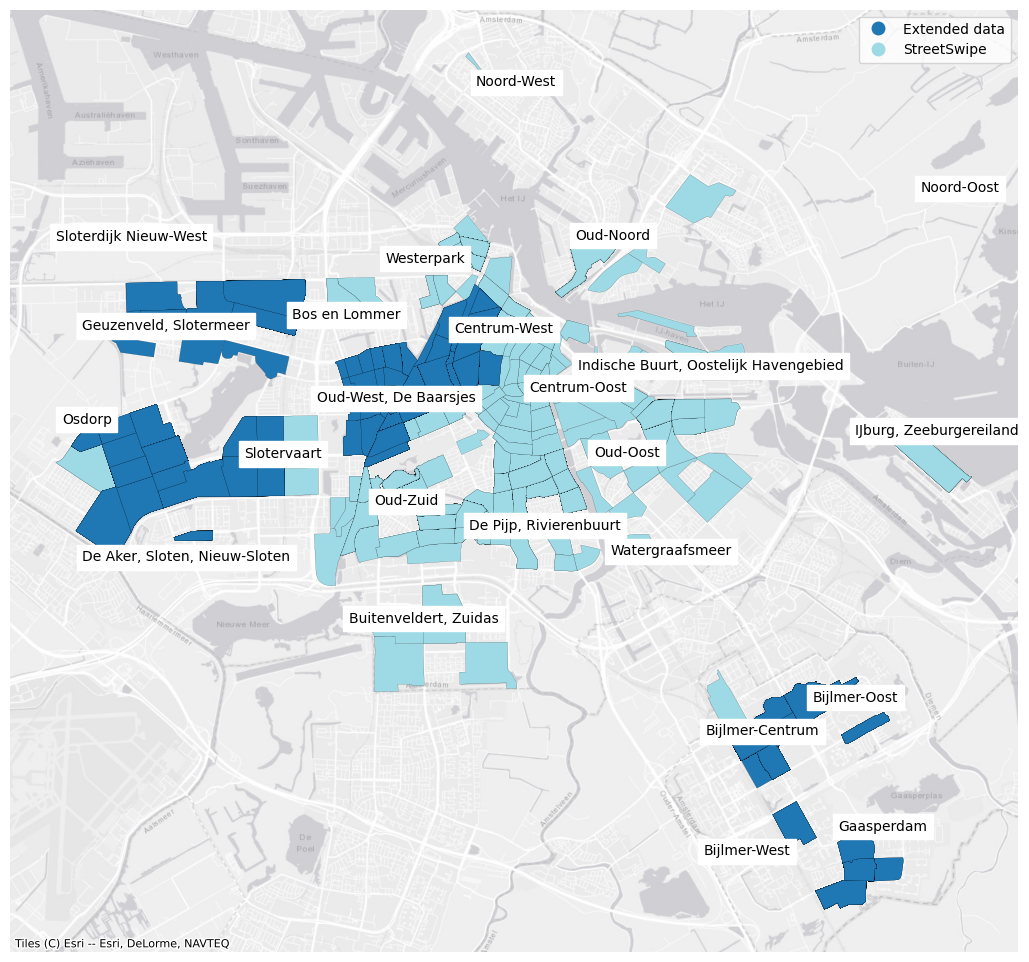
\includegraphics[width=0.5\textwidth
]{media/methodology/map1.png}
    \setlength{\belowcaptionskip}{-10pt}
    \caption{Areas of Amsterdam present in StreetSwipe and the extended dataset. StreetSwipe had images mainly from the city center (Centrum-Oost and -West), Oost, and Zuid. The extended dataset had images taken from Centrum-West (Jordaan), Oud-West, De Baarsjes, Nieuw-West, Bijlmer, and Gaasperdam.}
    \label{fig:map}
\end{figure}

\subsubsection{StreetSwipe}
The main dataset was retrieved from the Street-Swipe project \cite{streetswipe}. These images were originally from Google Street View, and was cropped to focus on facades (examples can be seen in Figure \ref{fig:SS_example}. Using crowd-sourcing, the project lets people decide whether each Amsterdam facade is gentrified, by voting "Yes" (gentrified) or "No" (non-gentrified) on the street view images of these facades. The official \textit{Gentrified} and \textit{Non-gentrified} labels for each facade are based on what the majority voted for. Thus, this dataset represents common visual perception of gentrification. Additionally, if subsequent voters decide against the majority (e.g. voting \textit{Gentrified} for a non-gentrified-labelled facade), they are also prompted to provide a textual reasoning for their decision. These mismatch responses were also available, however was out of scope of the study. 

\begin{figure}
    \begin{tabular}{cccc}
        \subfloat{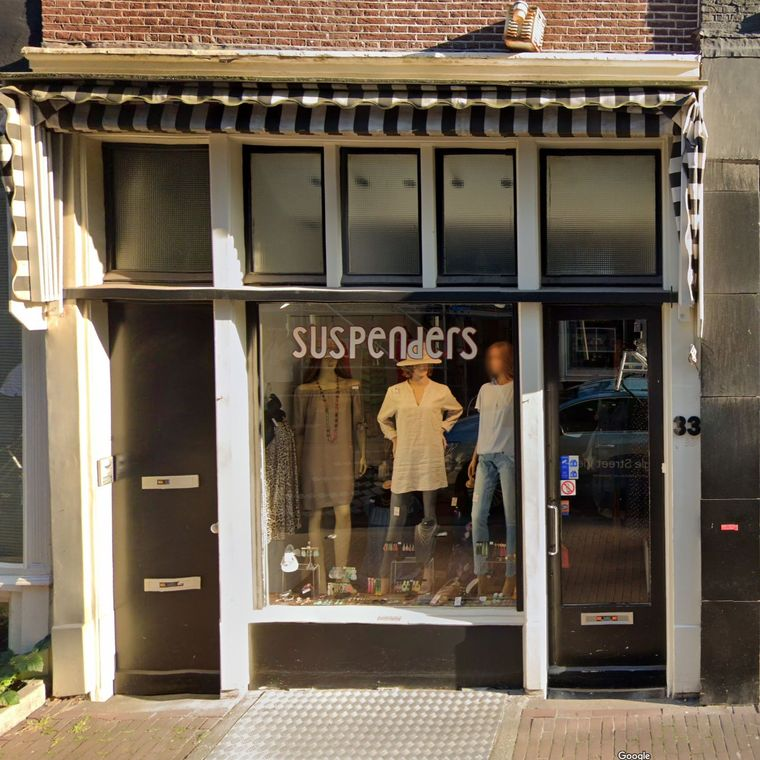
\includegraphics[width = 1.55in]{media/methodology/data_ex/SS/gen1.jpg}} &
        \subfloat{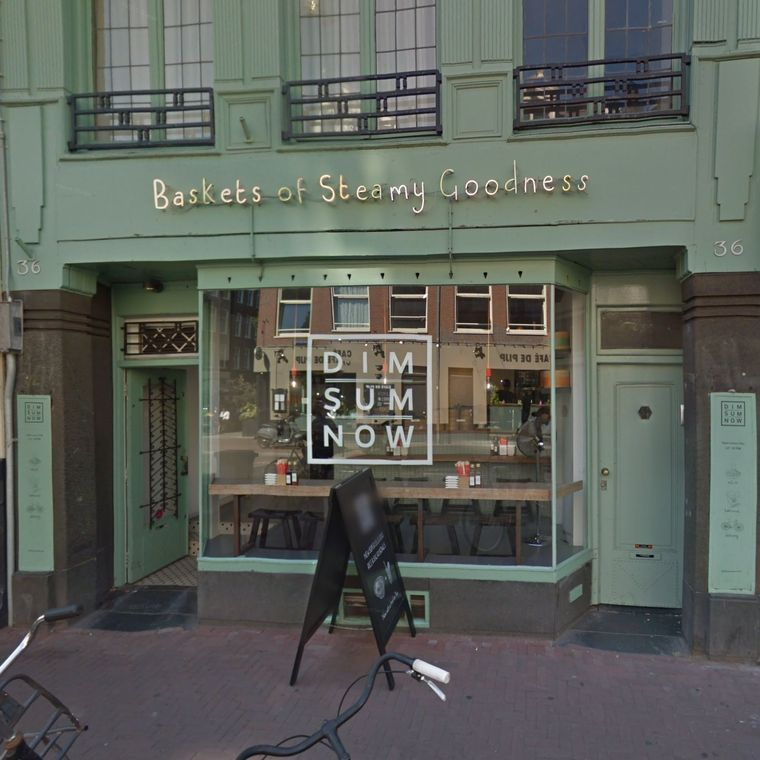
\includegraphics[width = 1.55in]{media/methodology/data_ex/SS/gen2.jpg}} \\
        \subfloat{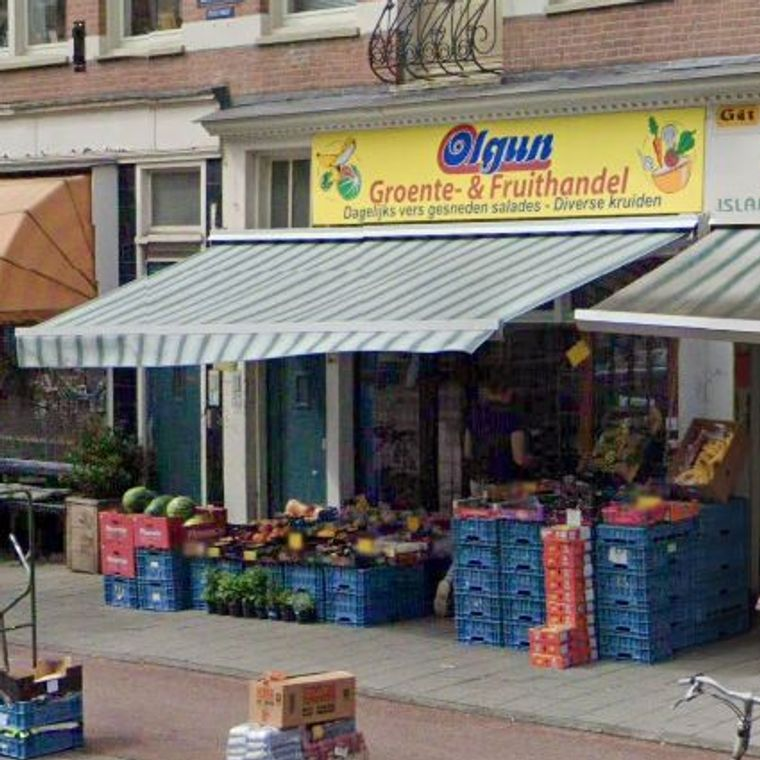
\includegraphics[width = 1.55in]{media/methodology/data_ex/SS/non1.jpg}} &
        \subfloat{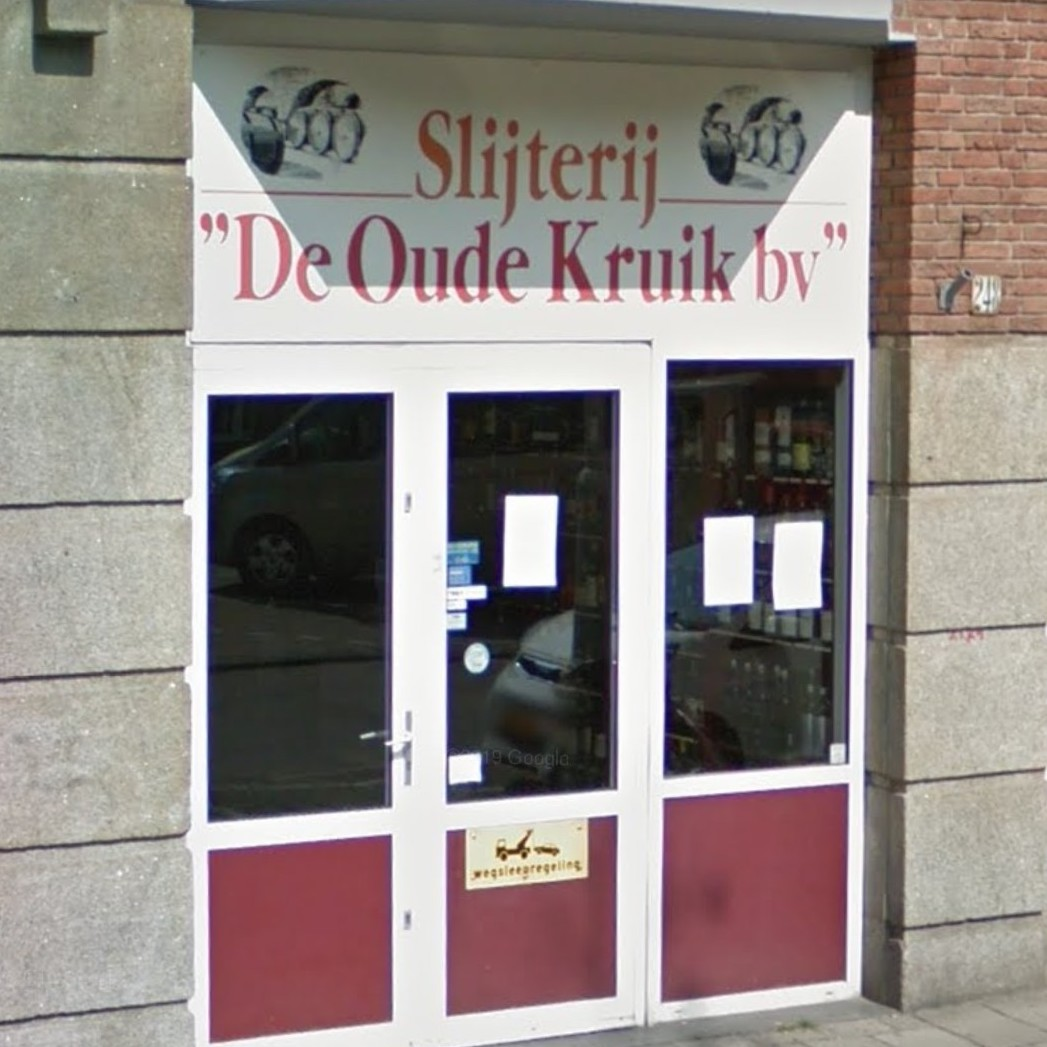
\includegraphics[width = 1.55in]{media/methodology/data_ex/SS/non3.jpg}} \\
    \end{tabular}
    \caption{Examples of StreetSwipe images.}
    \label{fig:SS_example}
\end{figure}

Since there are two versions of StreetSwipe, the data retrieved existed in two sets, consisting of 1912 higher resolution images from the older version and 529 lower resolution images from the new one. The StreetSwipe dataset thus had 2,441 images in total, each with its numbers of "Yes" and "No" votes, and metadata on the facade's location (latitude and longitude) and street name. The new version's images also had more detailed address, name, and type of business/services. There were also more votes in the new version than in the old one. The images from the old version were available directly, while the new ones were provided via URLs to a Google APIs bucket, and thus were scraped.

Feature engineering was done to create the gentrified/ non-gentrified label per image, by taking the vote higher in volume. The images were then re-grouped per their corresponding labels. There was class imbalance in the data, with 71\% of the images labelled non-gentrified (1731 images; versus 710 gentrified images). The images had quite consistent aspect ratios of approximately 1:1; however, they varied in size, ranging from around 300x300 to 1700x1700, with one outlier of size approximately 2500x1300.


\subsubsection{Extended data}
The images were retrieved as panoramas, along with corresponding front, back, left, and right views of the vehicle already extracted (Appendix \ref{sec:apx:appendix1} shows an example). Experiments were done with the text detection model to determine which version of the images would return signage with the least amount of noise. It was determined that passing the panoramas directly through the model returned the most noise (e.g. rows of windows, traffic signs), while the left and right views of the vehicle returned the least noise. Therefore, the left- and right-view images are used in the study. Figure \ref{fig:panolr_example} shows some example images.

Having selected gentrified and non-gentrified neighborhoods per existing literature, images were grouped per class and labelled accordingly. This dataset thus represents gentrification according to census data (irregardless of how a facade might be visually perceived). In total, this dataset contains 9340 images, with 5374 gentrified images (58\%) and 3966 non-gentrified (42\%). All images have size 512x512.

\begin{figure}
    \begin{tabular}{cccc}
        \subfloat{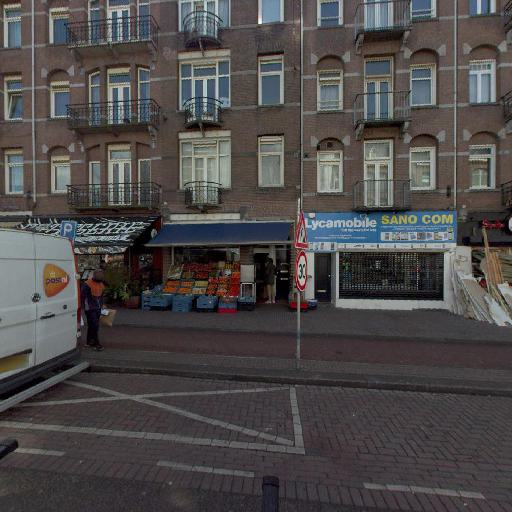
\includegraphics[width = 1.55in]{media/methodology/data_ex/extended/_left (2).jpg}} &
        \subfloat{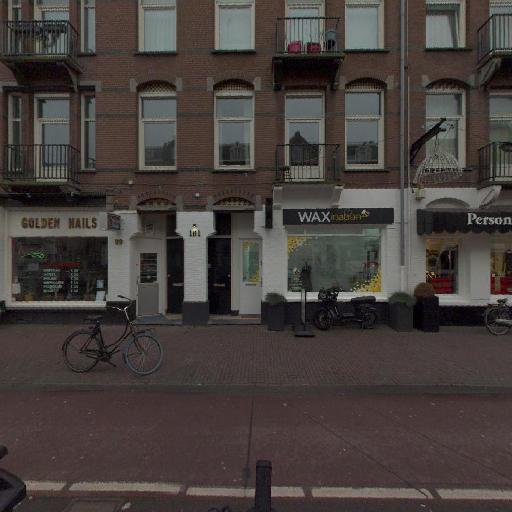
\includegraphics[width = 1.55in]{media/methodology/data_ex/extended/_left (4).jpg}} \\
        \subfloat{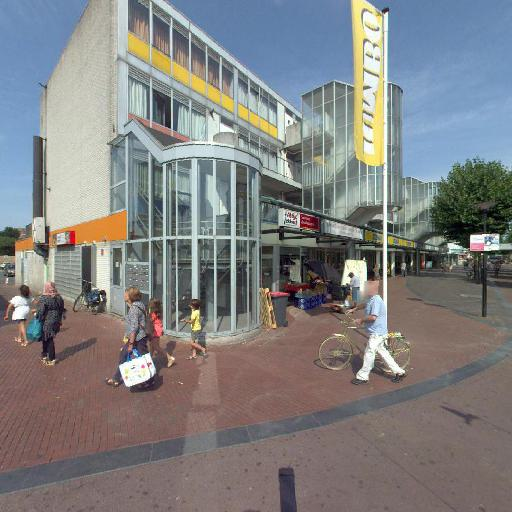
\includegraphics[width = 1.55in]{media/methodology/data_ex/extended/_right (1).jpg}} &
        \subfloat{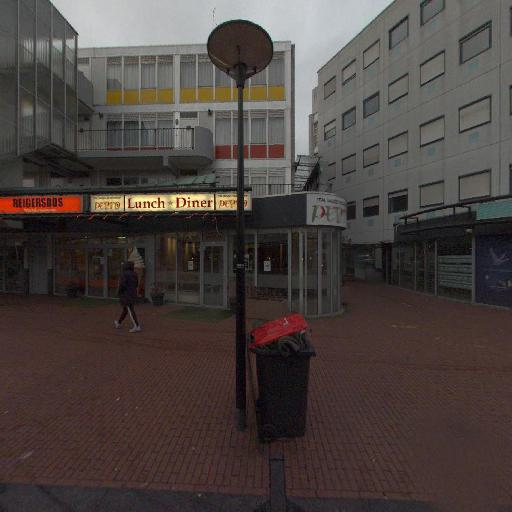
\includegraphics[width = 1.55in]{media/methodology/data_ex/extended/_right (2).jpg}} \\
    \end{tabular}
    \setlength{\belowcaptionskip}{-10pt}
    \caption{Examples of left- and right-view images from the extended dataset.}
    \label{fig:panolr_example}
\end{figure}


\subsection{Experimental setup}

The data pipeline is visualized in Figure \ref{fig:pipeline}. This section outlines the implementations of CRAFT and the ResNets.

\begin{figure*}
    \centering
    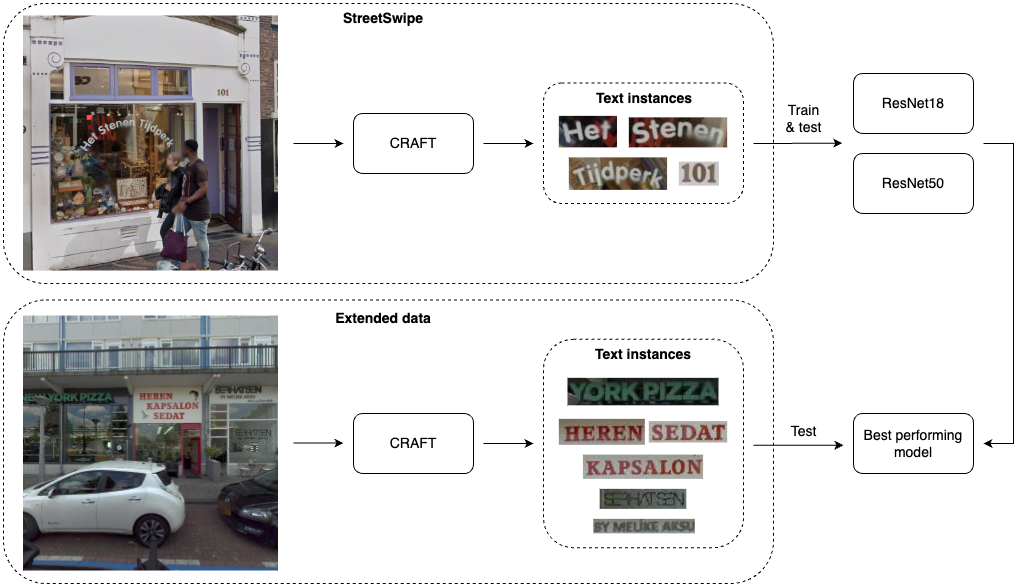
\includegraphics[width=0.9\textwidth]{media/methodology/Pipeline.png}
    \caption{Pipeline: Images of facades were first fed into the text detection model CRAFT to extract text instances. The ResNets were then trained and tested on instances from StreetSwipe. Subsequently, the best performing model was tested on instances from the extended data.}
    \label{fig:pipeline}
\end{figure*}


\subsubsection{Scene-text detection - CRAFT}

The first task is to detect and extract signage in the images of both datasets, using the pre-trained CRAFT model via the EasyOCR Python package.

More specifically, the \textit{detect} method was used, with text confidence threshold \textit{(text\_threshold)} set to 0.75, bounding box extension \textit{(add\_margin)} set to 0, and all other parameters set to their default values.

Text instances are cropped out by their bounding boxes and grouped per image, per class. 

Passing StreetSwipe through the CRAFT text detection model returned 10079 instances in total, with 2610 gentrified instances (26\%) and 7469 non-gentrified instances (74\%). The instances varied a lot in size, typically with width larger than height. The widths ranged from 8 to 1576, and heights ranged from 6 to 795 (see Appendix \ref{sec:apx:appendix2} - Figure \ref{fig:SS_ins_sz} for a visualization of the distributions). These text instances were used to train and optimize the classifier.

Passing the extended dataset through the text detection model returned 2473 instances in total, with 1633 gentrified instances (66.03\%) and 840 non-gentrified instances (33.97\%). The instances varied in size, typically with width larger than height. The widths ranged from 8 to 510, and heights ranged from 4 to 191 (see Appendix \ref{sec:apx:appendix2} - Figure \ref{fig:pano_ins_sz} for a visualization of the distributions). These text instances were used to test the classifier for generalizability.


\subsubsection{Classification - ResNet}

In order to train and optimize the ResNets on StreetSwipe text instances, the data was split into training, validation and test sets with 80:10:10 ratio. The data was randomly shuffled prior to splitting to maintain class distribution per split. Table \ref{tab:data_split} shows the size of each split in the data as well as class distributions.

{
\setlength\intextsep{0pt}
\begin{table}
    \begin{tabular}{lrrrl}
    \toprule
            & \multicolumn{1}{r}{Total} &\multicolumn{1}{r}{Gentrified} & \multicolumn{1}{r}{Non-gentrified} \\ \cline{1-4}
Train       & 8063                      & 2092 (25.95\%)                & 5971 (74.05\%)      \\
Val         & 1008                      & 238 (23.61\%)                 & 770 (76.39\%)       \\
Test        & 1008                      & 280 (27.78\%)                 & 728 (72.22\%)       \\
    \bottomrule
    \end{tabular}
    \caption{Sample size per data split, per class}
    \label{tab:data_split}
\vspace{-10pt}
\end{table}
}

Model training was done in PyTorch. Both the ResNet18 and ResNet50 were initialized with pre-trained ImageNet1K-V1 weights, with the final fully connected layer modified to give outputs of size 2. As a baseline, all the weights in the model were frozen and only the final layer was optimized; and no action was taken to account for class imbalance. Learning rate was set to 0.001, batch size was 32, and the model was trained for 50 epochs.

Next, the models were fine-tuned. PyTorch's WeightedRandomSampling was applied, with each class' weight calculated as 1/(class size). The loss function used was the cross entropy loss. The optimizer was stochastic gradient descent with a 0.9 momentum. StepLR learning rate decay scheduler was also implemented with a step size of 7 and gamma of 0.1. Hyperparameters tuning was done on the learning rate, batch size and number of training epochs.

\subsubsection{Visual inspection of model's output}
Random samples of the model's classification output were taken from each of the following subsets:

\begin{itemize}
    \item StreetSwipe's correctly classified signage per class with classification probability of 80\% and above.
    \item StreetSwipe's mis-classified signage, categorized by high ($ \geq 80\% $) and low (50-70\%) classification probability.
    \item Extended data's signage per class with classification probability of 80\% and above (irrespective of ground truth labels).
\end{itemize}


\subsection{Evaluation}

Performance metrics - namely accuracy, precision, recall, and F1 score - were calculated for the classifier in validation and testing. The macro-averaged metrics were used to compare models per epoch, and additionally metrics per class were calculated. The metrics were implemented using torchmetrics' MulticlassAccuracy, MulticlassPrecision, MulticlassRecall, and MulticlassF1Score. torchmetrics' ClasswiseWrapper was used to obtain metrics per class.

% The formulas are as follow:

% \begin{align*}
%     Accuracy = \frac{TP+TN}{TP+TN+FP+FN} \\
%     Precision = \frac{TP}{TP+FP} & Recall = \frac{TP}{TP+FN} \\
%     F1 Score = \frac{2 * Precision * Recall}{Precision + Recall}
% \end{align*}

